\newpage
\section{Surfen im Internet - Wie anonym ist anonym?}
Wenn man im Internet surft, hat man grundsätzlich das Gefühl, dass man alleine ist.
Man sitzt vor dem Computer, Tablet oder Smartphone und bedient den Webbrowser, der einem im Gegenzug die Informationen liefert, die man angefragt hat.
Abgesehen von Freunden oder sonstigen Leuten, die einem vielleicht über die Schulter schauen, scheint man privat unterwegs zu sein.
Diese Annahme ist aber falsch, denn \textit{das Internet} ist sich sehr wohl darüber bewusst, wer wann wo unterwegs ist.
Um zu verstehen, wie man sich  mehr Anonymität verschaffen kann, müssen zuerst gewisse Bestandteile und Funktionsweisen des Internets bekannt sein.
\\
Kleine Anmerkung am Rande: Mit Internet ist das \textit{World Wide Web} (WWW) gemeint. Dies schliesst beispielsweise E-Mail nicht mit ein.

\subsection{IP-Adressen und Domänennamen}
Das Internet besteht aus millionen von Computern und anderen Geräten, die miteinander vernetzt sind.
Auch der private Computer mit Internetzugang, den man für tägliche Arbeiten benutzt, ist ein Teil davon.
Jedes dieser Geräte hat nach aussen hin einen eindeutigen Identifikator, die sogenannte IP-Adresse.
Die IP-Adresse besteht aus mehreren Blöcken, die wiederum aus Zahlen (in Zukunft auch Buchstaben) bestehen.
Sie ist dabei immer eindeutig und wird einem vom Provider (z.B. Swisscom) zugeteilt.
Eine IPv4-Adresse könnte folgendermassen aussehen: 143.39.238.12
Die IP-Adresse wird aber nicht nur Privatanwendern zugewiesen, damit diese sich im Internet bewegen können.
Auch hinter \textit{www.google.ch} steckt eine IP-Adresse und genau so verhält es sich mit allen anderen Internetdiensten (Webseiten, Datei-Server, Download-Plattformen, etc.).
Jeder Dienst liesse sich über seine IP-Adresse ansprechen, sofern diese bekannt ist.
Da sich Menschen Namen aber deutlich leichter merken können, als Abfolgen von Zahlen, hat man das \textit{Domain Name System} (DNS) eingeführt.
Das DNS ist ein Verzeichnisdienst, der den Namensraum des Internets verwaltet und ist weltweit auf tausende von Server verteilt.
Seine Aufgabe besteht darin, sogenannte Domänennamen wie \textit{google.ch} in die zugehörigen IP-Adressen umzuwandeln\footnote{https://de.wikipedia.org/wiki/Domain\_Name\_System}.

\begin{figure}[h]
\centering
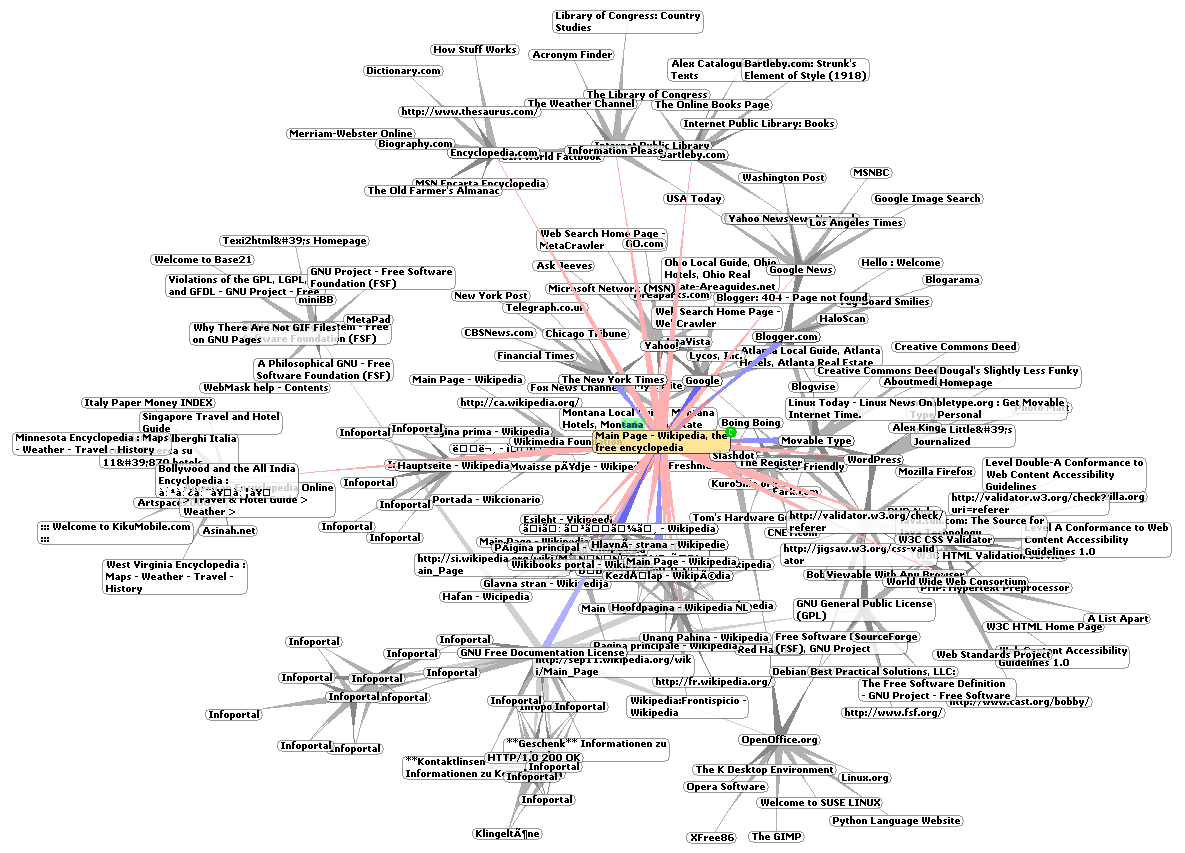
\includegraphics[scale=0.4]{images/wikipedia_www}
\caption{Webseiten im WWW um en.wikipedia.org}
\end{figure}

\newpage
\subsection{Server und Client}
Aus den obigen Erklärungen lässt sich ableiten, dass sich hinter einem Internetdienst immer auch ein Computer bzw. Server befinden muss.
Doch was ist ein Server eigentlich? Wikipedia gibt folgende Definition an:

\begin{quote}
\textit{Ein Server ist ein Computerprogramm oder ein Computer für den Zugriff auf eine zentrale Ressource oder Dienst in einem Netzwerk.}
\footnote{https://de.wikipedia.org/wiki/Server}
\end{quote}

Ein Server stellt also einen Dienst bereit, der vom sogenannten \textit{Client} benutzt werden kann.
Der Dienst ist beispielsweise eine Webseite, die vom Client - in diesem Zusammenhang dem Webbrowser - abgerufen und dargestellt wird.
Wie im vorherigen Abschnitt schon erwähnt, gibt es eine Vielzahl von verschiedenen Diensten und demnach auch eine Vielzahl von verschiedenen Servern.
Wenn es um Privatsphäre und Anonymität geht, stellen sich hier gleich mehrere Fragen:
Wem gehören diese Server?
Ist der Besitzer eines Servers gleichzeitig auch der Administrator?
Welche Informationen speichern die Server über seine Nutzer und geben sie diese weiter?
Welche Informationen können von den Server überhaupt eingesehen werden?
\\
Lediglich die letzte Frage lässt sich klar beantworten.
Diese verweist auch auf die Möglichkeiten, die man hat, die Privatsphäre im Internet zu erhöhen.
Zu den Spuren, die man im Internet hinterlässt, gehören unter anderem die IP-Adresse und damit zusammenhängend Informationen zum Provider und dessen Niederlassung.
Auch Informationen zum Browser inklusive dem verwendeten Betriebssystem können oft von den passierten Servern eingesehen werden.
Es gibt darüber hinaus viele verschiedene Technologien und Techniken, die es Servern erlauben, Nutzerinformationen abzuschöpfen (z.B. Cookies).
In diesem Kapitel liegt der Fokus aber auf den Verbindungsdaten - den IP-Adressen - und deren Anonymisierung.
An dieser Stelle setzt Tor an.

\subsection{Verbindungsdaten anonymisieren mit Tor}
Tor, ein Akronym für The Onion Routing, ist ein Netzwerk, welches geschaffen wurde, um Verbindungsdaten zu anonymisieren.
Um das Tor-Netzwerk zu verwenden, wird ein gleichnamiges Computerprogramme benötigt.
Dieses Programm ist frei, es sei denn, der Staat schränkt diese ein, wie es beispielsweise in China der Fall ist\footnote{http://www.technologyreview.com/view/427413/how-china-blocks-the-tor-anonymity-network/}.
Die Entwicklungen an Tor begannen 2002 an der Universität in Cambridge und dauern bis heute an. Der Quellcode der Software ist veröffentlicht und für jedermann einsehbar.
Global betrachtet nutzt wohl nur ein kleiner Teil der Leute Tor, da es erstens nicht sehr bekannt ist und zweitens die Nutzung mit einem gewissen Mehraufwand verbunden ist, der zusätzliches technisches Know-How verlangt. Im Rahmen der Enthüllungen von Edward Snowden hat Tor aber an Bedeutung und Verbreitung gewonnen. Die kritischen Stimmen wurden jedoch ebenfalls lauter und das zu Recht.

\subsection{Der zweifelhafte Ruf von Tor}
Tor hat einen zweifelhaften Ruf, der einen potenziellen Nutzer möglicherweise zwiegespalten zurück lässt.
Es heisst oft, dass im Tor-Netzwerk auf Grund der Anonymisierung verstärkt illegaler Handel getrieben wird.
Dies betrifft den Handel mit Drogen, Waffen und auch Kinderpornographie.\footnote{\url{http://www.zeit.de/digital/internet/2013-10/darknet-tor-netzwerk-vice}} \footnote{\url{http://www.nzz.ch/aktuell/digital/freedom-hosting-eric-eoin-marques-tor-1.18127905}}
Möchte man als gewissenhafter Nutzer tatsächlich mit solchen Tätigkeiten in Verbindung gebracht werden?
Was den zweifelhaften Ruf von Tor noch verstärkt, ist die Finanzierung des Projektes.
So wird die Weiterentwicklung von Tor bis heute zu grossen Teilen von militärischen Organisationen der USA sowie der US-amerikanischen Regierung  unterstützt.
\footnote{\url{https://de.wikipedia.org/wiki/Tor_\%28Netzwerk\%29\#Geschichte}}
\footnote{\url{http://www.heise.de/security/meldung/Neue-Diskussion-ueber-Finanzierung-des-Tor-Projektes-1955851.html}}
Dies grenzt beinahe schon an Ironie, sind es doch die amerikanischen Geheimdienste, die das Internet im grössten Masse aushorchen. Die Frage, die sich deshalb aufdrängt ist die Folgende: "Kann man überhaupt noch auf die anonyme Funktionsweise von Tor vertrauen oder muss man davon ausgehen, dass amerikanische Geheimdienste das Netzwerk bewusst aufgebaut haben, um jeden abzuhören, der offenbar etwas zu verstecken hat?"
\\
Kürzlich ist bekannt geworden, dass die Bemühungen der NSA, Nutzer vom Tor-Netzwerk gezielt zu de-anonymisieren, sehr ineffizient sind.\footnote{\url{http://www.heise.de/security/meldung/Neues-von-der-NSA-Tor-stinkt-1972983.html}}
Ist das eine bewusste Falschmeldung? Oder ist Tor vielleicht doch sicherer, als es den Anschein macht? Diese Frage lässt sich leider nicht abschliessend beantworten. Trotzdem sollte nicht ausser Acht gelassen werden, dass die Tor-Software ein Open Source Software ist, die aus vielen Fachkreisen befürwortet wird. Es lohnt sich deshalb, die Funktionsweise von Tor zu analysieren, um mehr Substanz für ein Urteil zu gewinnen.

\subsection{Wie funktioniert Tor?}
Der Name \textit{The Onion Routing} kommt nicht von ungefähr. Die verwendete Anonymisierungstechnik \textit{Onion-Routing} lässt auf Grund ihrer Funktionsweise Vergleiche mit einer Zwiebel zu. Im folgenden soll diese genauer erklärt werden. Dazu müssen aber zuerst ein paar Begriffe genauer ausgeführt sein:
\begin{itemize}
\item Client: Computerprogramm, das auf dem Rechner des Nutzers installiert und verwendet wird
\item Tor-Server: Rechner im Tor-Netz, dessen Aufgabe es ist, Daten bzw. Anfragen zu empfangen und diese anschliessend an einen neuen Tor-Server weiterzuleiten
\item Entry-Guard: Erster Tor-Server in der Kaskade, der die Daten bzw. die Anfrage direkt vom Nutzer bekommt und diesen somit noch kennt
\item Exit-Node: Letzter Tor-Server in der Kaskade, der als Endpunkt auftritt und die Daten bzw. die Anfrage an das gewünschte Ziel weiterleitet
\end{itemize}

Im Folgenden werden die verschiedenen Stationen bzw. Phasen der Prozedur genauer beschrieben. Man bekommt vielleicht das Gefühl, dass der Ablauf zeitintensiv und aufwendig ist. Tatsächlich handelt es sich aber von Start bis Ende des Ablaufs lediglich um Millisekunden bzw. Sekunden. Das Ganze hängt natürlich auch immer von der eigenen Verbindungsgeschwindigkeit, der konkreten Anwendung und der Performanz des Tor-Netzwerks ab.

\begin{enumerate}
\item Um Tor überhaupt nutzen zu können, muss als erstes der  Client (Onion-Proxy) gestartet werden.
\item Dieser verbindet sich automatisch mit dem Tor-Netzwerk und lädt eine Liste aller nutzbarer Tor-Server herunter.
\item Ist die Liste komplett, entscheidet sich der Client für eine zufällige Route über die Tor-Server.
\item Er baut nun eine verschlüsselte Verbindung mit dem ersten Tor-Server (Entry-Guard) der Route auf und sendet ihm die Daten.
\item Der Entry-Guard verschlüsselt die Daten erneut und sendet diese an einen weiteren Tor-Server.
\item Dieser tut genau das Gleiche noch einmal, worauf die Daten schliesslich zum letzten Server (Exit-Node) kommen.
\item Der Exit-Node entschlüsselt die Daten und leitet sie zum gewünschten Ziel weiter. Das ist die einzige Strecke im ganzen Ablauf, auf der die Daten nicht mehr verschlüsselt weitergeleitet werden.\footnote{\url{https://www.torproject.org/about/overview.html.en\#thesolution}}
\footnote{\url{https://de.wikipedia.org/wiki/Tor_\%28Netzwerk\%29\#Anonymes_Surfen}}
\end{enumerate}

Die versendeten Daten werden im Laufe der Kaskade in mehrere Verschlüsselungsschichten verpackt, damit die passierten Tor-Server nicht sehen können, worum es sich dabei handelt. Daher kommt auch der Name der Prozedur. Der finale Aufbau des Pakets gleicht einer Zwiebel mit mehreren Schichten, die  schlussendlich wieder entpackt werden müssen. Diese Aufgabe übernimmt dann, wie schon erwähnt, der Exit-Node. Generell gilt, dass die Daten immer drei Tor-Server passieren. Da die Tor-Server jeweils nur die Rechner links und rechts von sich kennen, weiss nur der erste Tor-Server über die Identität des Nutzers Bescheid. Der dritte und letzte Tor-Server kennt dann nur noch den Tor-Server, der ihm die Daten weitergeleitet hat, die Daten selbst und das finale Ziel.\footnote{\url{https://de.wikipedia.org/wiki/Onion-Routing\#Verschl.C3.BCsselungsschema}}
Die zufällig gewählte Route wird vom Tor-Client ungefähr alle zehn Minuten gewechselt. So soll eine möglichst hohe Sicherheit gewährleistet werden. Gefährlich wird es für den Nutzer dann, wenn jemand Eintritts- und Austrittsknoten kontrolliert. Die Anonymität wäre dann aufgehoben, da der \textit{Lauscher} Ursprung, Ziel und Inhalt der Daten kennt.

\begin{figure}[h]
\centering
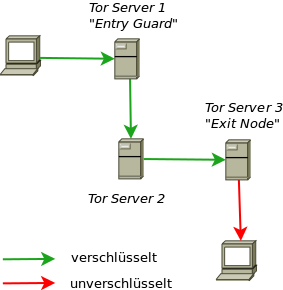
\includegraphics[scale=0.7]{images/tor}
\caption{Tor}
\end{figure}

Soll Tor benutzt werden, müssen weitere Regeln beachtet werden, die es für eine erfolgreiche Anonymisierung einzuhalten gilt:
\begin{itemize}
\item Wann immer möglich, eine verschlüsselte Verbindung aufbauen (HTTPS)
\item Soziale Netzwerke vermeiden, da sie die Identität preisgeben
\item Web-Extensions, wie Java-Script und Flash-Cookies vermeiden (beides Technologien für spezielle Funktionalitäten und Multimediainhalte im Web)
\item Keine persönlichen Angaben machen in Webformularen und dergleichen
\item Tor nur dann benutzen, wenn es auch wirklich Sinn macht
\end{itemize}

Der letzte Punkt ist sehr wichtig, da die Anonymität durch Protokollierung gebrochen werden kann. Protokolliert ein Tor-Server genügend lang die passierenden Daten, kann nach durchschnittlich sechs Monaten die Identität aufgedeckt werden. Je öfter man den Dienst also braucht, desto mehr Informationen gibt man dem vermeintlichen Schnüffler. Die Zeit bis zum Aufdecken der Identität ist dabei stark von der Infrastruktur abhängig. Staatliche Behörden mit immensen Rechenzentren hätten folglich keine grossen Probleme damit, die Anonymität von beobachteten Nutzern nach kurzer Zeit aufzuheben.\footnote{\url{http://www.heise.de/security/meldung/Tor-Benutzer-leicht-zu-enttarnen-1949449.html}}

\subsection{Vor- und Nachteile}
Tor ermöglicht dem Nutzer, sich anonym im Netz zu bewegen. Die Einrichtung des Dienstes ist dabei relativ simpel und schnell erledigt. Nachteilig daran ist, dass das \textit{Surferlebnis} relativ stark eingeschränkt ist, also viele Multimediafunktionalitäten nicht gleichzeitig genutzt werden können. Auch die Geschwindigkeit, mit der man im Netz unterwegs ist, ist geringer als ohne Tor. Auch hier ist es wieder eine Frage der Prioritäten. Eine grössere Verbreitung und Unterstützung von Tor würde hier aber teilweise Abhilfe schaffen. Man muss sich vielleicht einfach noch etwas gedulden. Auch sollte man sehr bewusst mit Tor umgehen. Man macht sich möglicherweise automatisch verdächtig durch die Benutzung des Dienstes und sollte auch nicht vergessen, wer der finanzielle Hauptsponsor des Projektes ist.
Nachfolgend werden die Vor- und Nachteile noch einmal kurz aufgelistet.
\\
\\
Vorteile
\begin{itemize}
\item Relativ sicher, was Anonymität betrifft
\item Einfach einzurichten
\item Open-Source
\item Kostenlos
\end{itemize}

Nachteile
\begin{itemize}
\item Starker Zusammenhang mit amerikanischen Behörden (finanz. Unterstützung)
\item Schlechter Ruf
\item Bei falscher Anwendung ineffektiv
\item Noch relativ langsam
\item Nutzung von Multimediafunktionalitäten im Web eingeschränkt
\end{itemize}

\subsection{Experiment}

\subsubsection{Zielsetzung}
Das Ziel war es, einen Computer in einen Access Point umzuwandeln und auf diesem Tor aufzusetzen.
Der Access Point hat dabei die Aufgabe, jedes Gerät, das sich mit ihm verbindet, über das Tor-Netzwek ins Internet weiterzuleiten und so eine Anonymisierung der Verbindungsdaten zu ermöglichen.
Als Computer kam ein Raspberry Pi zum Einsatz.
Es handelt sich dabei um einen Einplatinen-Computer mit beschränkten Ressourcen, der sich vor allem wegen seiner geringen Grösse sehr gut für dieses Experiment eignete.
Einzelheiten dazu sind im Handbuch beschrieben.
Als Betriebssystem wurde eine für den Pi angepasste Version von Debian mit dem Namen Raspbian verwendet.
Es handelt sich dabei um eine Linux-Distribution, die jedermann frei herunterladen und benutzen kann.

\subsubsection{Installation}
Die erste Hürde bei dem Experiment war die Wahl des WLAN-Adapters, welcher für die Access Point-Funktionalität benötigt wird. Nicht jeder Adapter kann in den \textit{Access Point Mode} versetzt werden, weshalb zuerst ein kompatibles Gerät ausfindig gemacht und bestellt werden musste. Die restlichen Komponenten, die vor allem für den Betrieb des Raspberry Pis gebraucht werden, waren bereits vorhanden und schnell eingerichtet. Die Installation selbst ging funktionierte ohne grosse Probleme. Man kann diese grob in zwei Schritte aufteilen. Der erste Schritt, das Einrichten des Raspberry Pis als Access Point, ist der aufwendigere der beiden und es gab diverse Konfigurationen, die vorgenommen werden mussten. Der zweite Schritt, das Installieren und Einrichten von Tor, war schnell erledigt und stellte keine grossen Probleme mehr dar. Allgemein ist die Installation kein grosse Problem, da es im Internet eine Menge Anleitungen und Hilfestellungen gibt, auf die man zurückgreifen kann. Beim anschliessenden Testen des Tor Access Points wurde noch die eine oder andere Einstellungsmöglichkeit entdeckt, die die Sicherheit von Tor zusätzlich erhöhen.

\subsubsection{Fazit}
Das Einrichten von Tor war gut bewältigbar und spannend dazu. Anhand von Hilfestellungen und Anleitungen im Internet liessen sich auch die oben beschriebenen Probleme lösen. Die angeschaffte Hardware - Raspberry Pi und Zubehör - kostete knapp unter 100 Franken. Wenn man Tor ausprobieren möchte, ohne die Software auf seinem Produktivsystem zu installieren, sollte auf diese Variante zurückgreifen. Mehr Informationen dazu finden sich im Handbuch.
\\
An dieser Stelle kann der Einsatz von Tor nicht uneingeschränkt empfohlen werden. Dazu gibt es schlicht zu viele Ungereimtheiten. Ausprobieren und Kennenlernen lohnt sich aber allemal. Man kann viel dabei lernen und evtl. gibt es in Zukunft klarere Antworten auf die vielen Fragen, die sich im Zusammenhang mit Tor stellen. Es gibt zudem Möglichkeiten, bestimmte Risiken zu minimieren. Auch dazu findet man detaillierte Informationen im Handbuch.
\\
Das Handbuch befindet sich im Anhang zu diesem Dokument oder einzeln unter: ...xyz

%Quellen:
%https://de.wikipedia.org/wiki/Tor_\%28Netzwerk\%29
%https://de.wikipedia.org/wiki/Client
%https://de.wikipedia.org/wiki/Onion-Routing
%https://www.torproject.org/about/overview.html.en
%https://de.wikipedia.org/wiki/United_States_Naval_Research_Laboratory
%http://www.heise.de/security/meldung/Neues-von-der-NSA-Tor-stinkt-1972983.html

%http://www.spiegel.de/netzwelt/netzpolitik/botnetz-anonymisierungsdienst-tor-unter-beschuss-a-921643.html
%http://www.heise.de/security/meldung/Neue-Diskussion-ueber-Finanzierung-des-Tor-Projektes-1955851.html
%http://www.heise.de/security/meldung/Tor-Benutzer-leicht-zu-enttarnen-1949449.html
